\chapter{Introduction}
\label{sec:introduction}

After a drop in rail passenger transport in 2020, it quickly recovered and increased by almost 71\%, resulting in 328,3 million passengers in 2023 \cite{schienenpersonenverkehrAustria}.
The Wiener Linien and the ÖBB show similar behaviors with an increase of 218 million and 115,4 million passengers from 2020 to 2023 respectively \cite{wienerLinienAustria} \cite{oebbAustria}.

The increase in train traffic is bound to a rise in accidents.
In Austria, 34 rail traffic accidents with 38 victims were recorded in 2021.
Of them 24 were seriously injured and 14 were killed \cite{verkehrstatistik2022}.
Incidents include a train derailment in the area of a signal box, where there usually are many switches \cite{zugEntgleist}.
In 2022 in Münchendorf a train drove too fast over a switch, resulting in a derailment accident, with one passenger dead and 25 injured \cite{zugUnfall1Tod}.
Also in other countries like the Czech Republic, an accident occurred, where a head-on collision of two trains resulted in four deaths.
It is suspected that an incorrect switch caused that incident \cite{zugUnfallFrontal}.
The cause of all accidents mentioned can be traced back to either an incorrect set switch or a derailment at a switch.
This leads to the idea that correctly identifying the switch states may have prevented these accidents.

% Bild von Zugunfällen Münchendorf und Tschechien
\begin{figure}[H]
    \centering
    \begin{subfigure}{0.48\textwidth}
        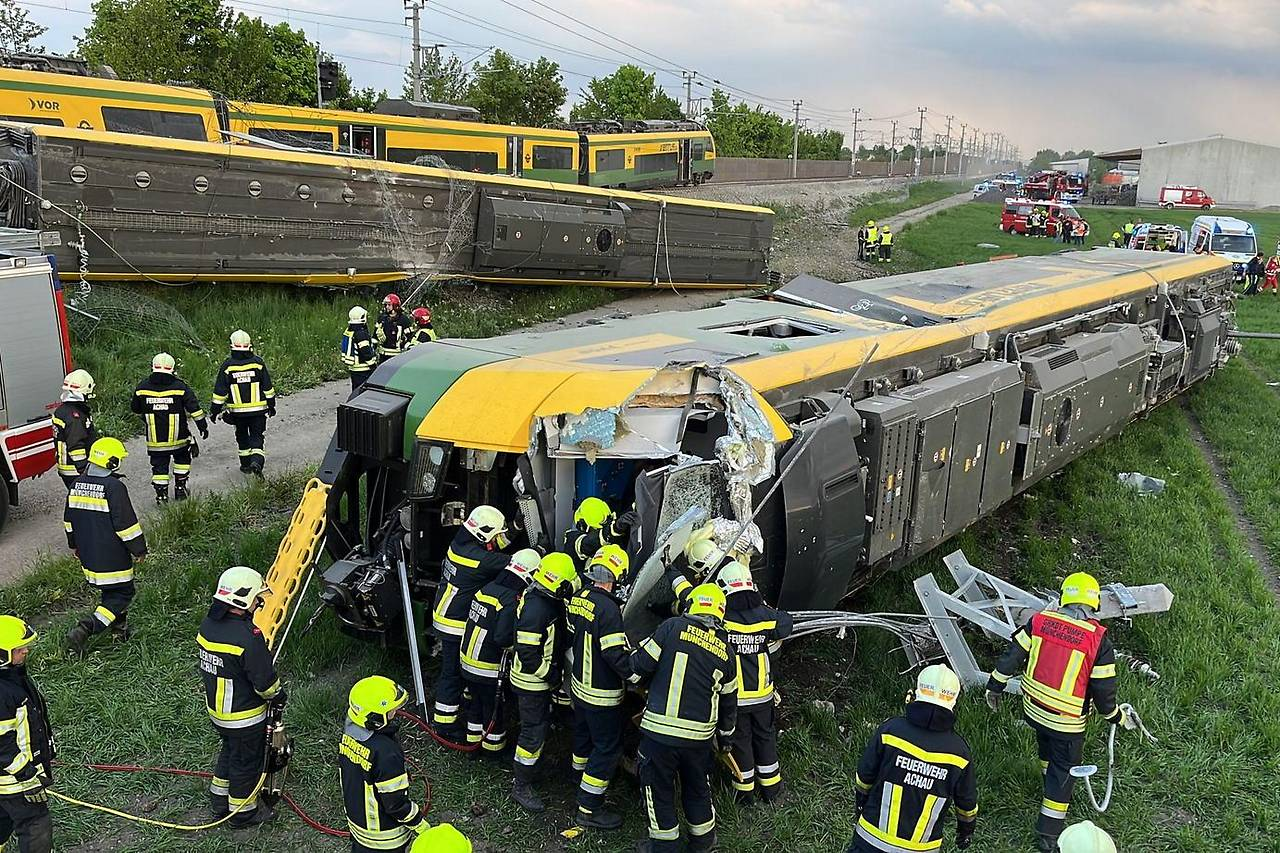
\includegraphics[width=\linewidth, height=5cm, keepaspectratio]{PICs/Introduction/unfallMuenchedorf.jpg}
        \caption{Accident in Münchendorf, Austria. The train drove too fast over a switch and derailed, resulting in one death and 25 injured. \cite{zugUnfall1Tod}}
        \label{fig:unfallMuenchedorf}
    \end{subfigure}
    \hfill
    \begin{subfigure}{0.48\textwidth}
        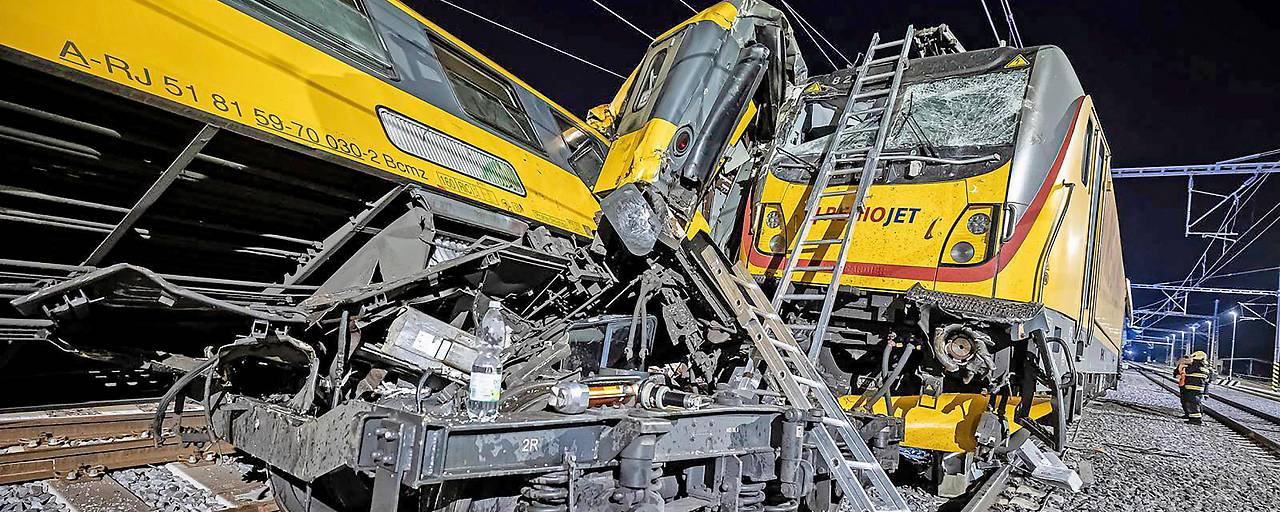
\includegraphics[width=\linewidth, trim={13cm 0cm 5cm 0cm}, clip]{PICs/Introduction/unfallTschechien.jpg} % trim={left bottom right top}
        \caption{Accident in the Czech Republic. Head-on collision of two trains. The suspected cause is an incorrecty set switch, resulting in four deaths. \cite{zugUnfallFrontal}}
        \label{fig:unfallTschechien}
    \end{subfigure}
    \caption{Train accidets in \textbf{(a)} Austria and \textbf{(b)} the Czech Republic, where misinformation of switches resulted in deaths.}
    \label{fig:zugUnfaelle}
\end{figure}

Simultaneously, autonomous vehicles are becoming increasingly seen as revolutionary technology for the future \cite{FraunhoferInstituteforCognitiveSystemsIKS}.
Also indicated by the "Autonomous Vehicle Readiness Index" \cite{autonomousVehicleReadinessIndex} in most countries including Austria \cite{autonomousVehicleReadinessCounties}.
Especially autonomous road vehicles are rapidly evolving and could improve safety \cite{railsem19dataset} \cite{tepNet2024}, with machine-learning algorithms being a key trend \cite{railsem19dataset}.
The rail domain on the other hand, has gotten little attention \cite{railsem19dataset}.
This is because, unlike other modes of transportation like airplanes or cars, trains follow a predetermined path defined by the tracks.
Nevertheless, trams or other low-speed trains operate in dynamic environments where autonomous systems are still needed to respond to unpredictable events \cite{tepNet2024}.
Therefore autonomy for these modes of transport will gain importance in the future \cite{railNet2019}.

One particular task of an autonomous train system involves filtering out the area in front of the vehicle, which can be defined as the danger zone.
This area represents where the train is headed and the space, which is occupied next.

The problem is, that many state-of-the-art techniques in the rail domain consider all rails or rail tracks, and often make no distinction between the train's track and other tracks \cite{tepNet2024}.
This can be observed in figure \ref{fig:railSem19-images-denseLabels}, in the right two images of figure \ref{fig:railVID_dataset_images} and in figure \ref{fig:RailSet-Seg_example_image_GT}.
While the segmentation of rails can be used for obstacle detection \cite{railNet2019}, the output of these methods can easily be misinterpreted \cite{tepNet2024}.
Train infrastructure is complex, with multiple tracks often crossing, merging, or splitting at switches. Therefore, it is insufficient to recognize all tracks in a single image.
A more targeted system is needed, which only detects the train's track and predicts the upcoming path at switches \cite{tepNet2024}.
Such a system identifies the most relevant danger zone and when it is real-time capable it could be used as a preprocessing step for other algorithms or safety features \cite{tepNet2024} \cite{railNet2019}.
Leading to better-informed decisions \cite{tepNet2024}, possibly preventing accidents like the ones mentioned before and potentially save lifes.
Figure \ref{fig:train-ego-path} shows a schematic visualization of a more targeted system.

This is why in the line of this work a distinction between \textit{rail detection} and \textit{rail track prediction} is made.
On the one hand, \textit{rail detection} in this context is filtering out rails or rail tracks with no further information about the own or adjacent rails.
On the other hand, \textit{rail track prediction} answers the question of where the train will be in the next few moments, particularly when switches are present that split the track.
In figure \ref{fig:train-ego-path} a \textit{rail detection} would ouput both the green and the red marked tracks as one class and a \textit{rail track prediction} outputs just the green track.

\vspace{1cm} % Größerer Abstand zwischen den Reihen

\begin{figure}[H]
    \centering
    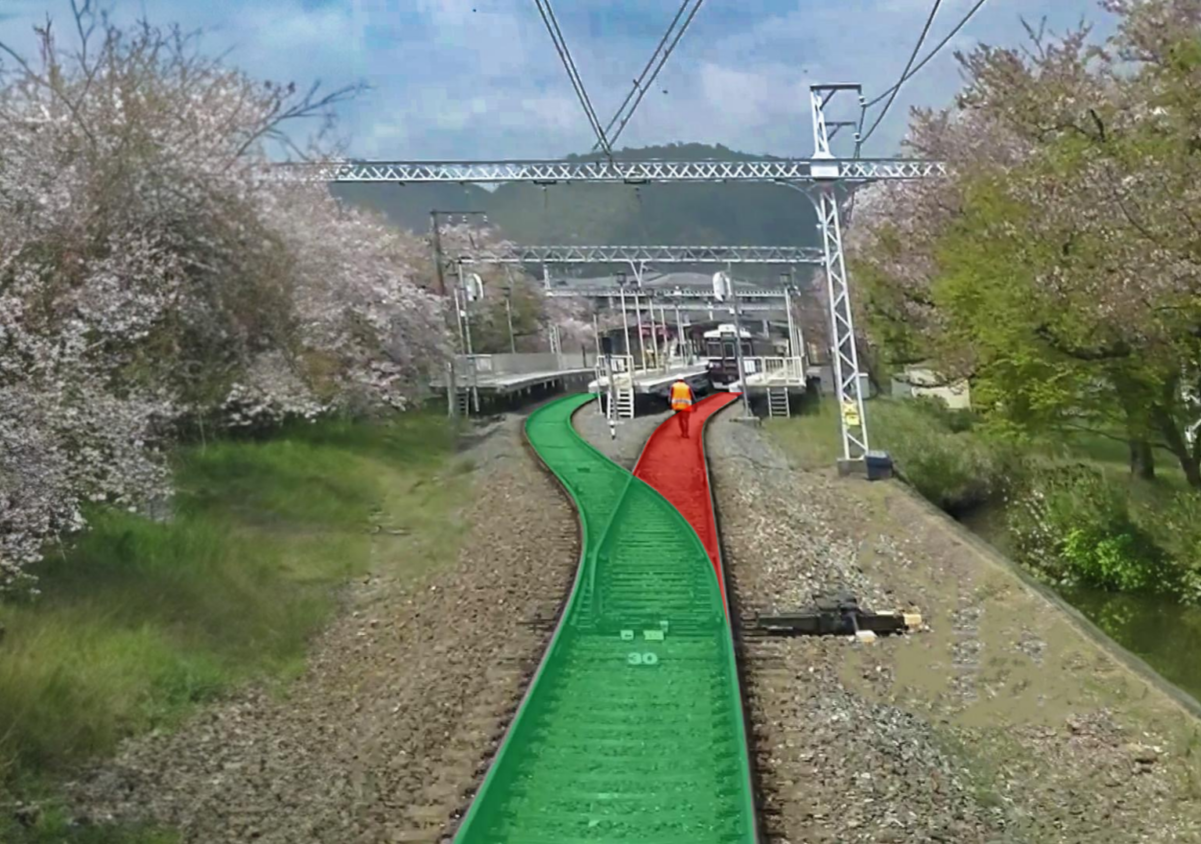
\includegraphics[width=0.5\linewidth]{PICs/Introduction/train-ego-path.png}
    \caption{Example of a diverging rail track at a switch. The trains path is marked in green. The path the train cannot take is marked in red. This path is be obstructed and would be unsafe \cite{tepNet2024}. \textit{rail detection}-output: green and red track; \textit{rail track prediction}-output: green track}
    \label{fig:train-ego-path}
\end{figure}

The focus of \textit{rail track prediction} extends beyond solely camera-based detection of the train's path.
It particularly emphasizes the accurate identification of switches where the train's path diverges, as illustrated in Figure \ref{fig:train-ego-path}.

Consequently, the goal of this work is the development of a rail track prediction system, which correctly predicts the most relevant danger zone and the direction in which the train is moving
This is done with an emphasis on scenarios involving track splits through switches present in the \ac{FOV}.
Since the use case primarily takes place in dynamic environments, another goal, besides achieving an acceptable accuracy, is to ensure it operates in real-time and is therefore lightweight \cite{tepNet2024}.

As the goal is to perceive the environment in front of the train, it is most advantageous to use front-view cameras \cite{tepNet2024} \cite{railNet2019}.
Images are captured in the driving direction from the driver's cabin because it is the best view of the tracks \cite{tepNet2024}.

The main contributions of this work can be roughly divided into three parts.

\begin{enumerate}
    \item Firstly, an initial approach was taken that aimed to combine object detection and semantic segmentation.
    However, due to unsatisfactory results, this methodology was deemed ineffective, leading to the pursuit of a fundamentally different solution.
    \item Secondly, \ac{TEP}-Net \cite{tepNet2024} was chosen as the new baseline for further experiments.
    Improvements are implemented with a specific focus on correct path prediction in the presence of switches.
    \item Thirdly, as further improvements were anticipated through the use of the temporal component with \ac{RNN}s, the system was adjusted to accept video information rather than single frames as input.
    Thus, the data loading logic was adapted and models were modified.
    Additionally, a temporal dataset was created.
    To minimize the workload for annotation, an auto labeler was developed utilizing the improved single-frame-based model.
\end{enumerate}

\vspace{2cm} % Größerer Abstand zwischen den Reihen

\textbf{\ref{sec:stateOfTheArt}} \textbf{\nameref{sec:stateOfTheArt}} describes different approaches, to how the train track prediction problem can be solved.
In this section, thorough research is done, which gives an overview of various approaches, models, and fitting datasets.
Additionally, a couple of papers that could serve as a baseline are discussed in more detail.
In \textbf{\ref{sec:methodology}} \textbf{\nameref{sec:methodology}} the used datasets as well as the hardware and software frameworks used for training and evaluation are described.
Additionally, this work includes the development of a temporal dataset with partly auto-labeled annotations.
The labeling process and algorithms for auto-labeling are also described in this section.
After that carried-out experiments are described in \textbf{\ref{sec:experiments}} \textbf{\nameref{sec:experiments}} and their results are described in \textbf{\ref{sec:results}} \textbf{\nameref{sec:results}} following a discussion in \textbf{\ref{sec:discussion}} \textbf{\nameref{sec:discussion}}.
In the final section \textbf{\ref{sec:conclusionAndOutlook}} \textbf{\nameref{sec:conclusionAndOutlook}}, the work is summarized and further possible ideas for improvements are presented.
